%It is without doubt that our understanding of how to build reliable systems out of unreliable components has led the development of robust and fairly reliable large-scale software and networking systems. The inherent instability of extreme-scale distributed systems of the future in terms of the envisioned high-rate and diversity of faults, however, calls for a reconsideration of the fault tolerance problem as a whole. % and the exploration of radically different approaches that go beyond adapting or optimizing well known and proven techniques.

Shadow Replication is a novel computational model that goes beyond adapting or optimizing well known and proven techniques, and explores radically different methodologies to fault tolerance~\cite{mills_2014_icnc,mills_2014_pdp,mills2014power}. % that scale to extreme-scale computing infrastructures. 
%The proposed solutions differ in the type of faults they manage, their design, and the fault tolerance protocols they use. %It is not just a scale up of  ``point" solutions, but an exploration of innovative and scalable fault tolerance frameworks. 
%When integrated, it will lead to efficient solutions for a ``tunable" resiliency that takes into consideration the nature of the data and the requirements of the application.
The basic tenet of Shadow Replication is to associate with each main process a suite of “shadows” whose size depends on the 
``criticality" of the application and its performance requirements. Each shadow process is an exact replica of the original 
main process, but it executes at a reduced rate to save power when possible.
Shadow Replication achieves power efficiency under QoS requirements by dynamically responding to failures. 
%If the main process completes the task successfully, the associated shadows will be terminated immediately. If the main process fails, however, one of the shadow processes will be promoted to be a 
%new main process, and possibly increase its execution rate to mitigate delay.

Assuming the fail-stop fault model, where a processor stops execution once a fault
occurs and failure can be detected by other processors~\cite{gartner_faults_1999,cristian_comm_1991}, 
the Shadow Replication fault-tolerance model can be described as follows:
\begin{itemize}
	\item A main process, $P_m(W,\text{ }\sigma_m)$, whose responsibility is to executes a task of size $W$ at a speed of $\sigma_m$;
	\item A suite of shadow processes, $P_{s}(W,\text{ }\sigma_b^s, \text{ }\sigma_a^s)$ ($1 \le s \le \cal S)$, where $\cal S$ is the size of the suite. The shadows execute on separate computing nodes. Each shadow process is associated with two execution speeds. All shadows start execution simultaneously with the main process at speed $\sigma_b^s$ ($1 \le s \le \cal S$). Upon failure of the main process, all shadows switch their executions to $\sigma_a^s$, with one shadow being designated as the new main process. This process continues until completion of the task.
\end{itemize}
%All shadows execute simultaneously with the main process at speed $\sigma_a^s$

\begin{figure}[!t]
	\begin{center}
		\subfigure[No Failure]
		{
			\label{fig:sc_no_fail}
			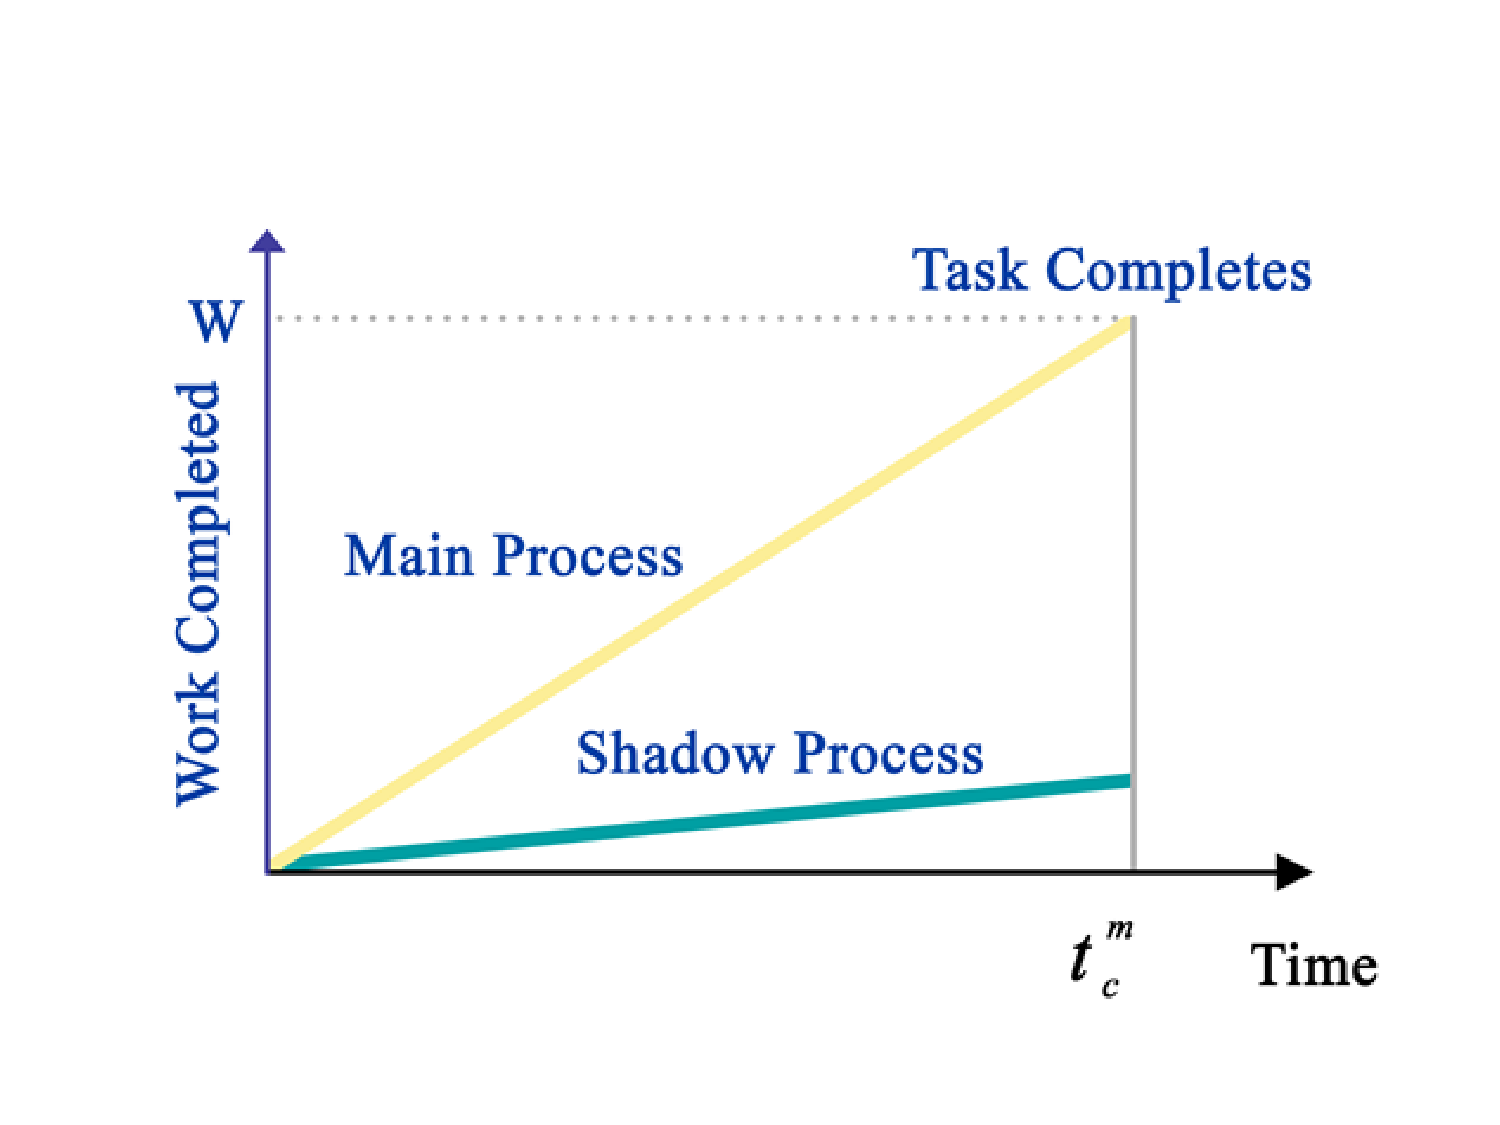
\includegraphics[width=0.31\textwidth]{figures/example1.pdf}
		}
		\subfigure[Shadow Process Failure]
		{
			\label{fig:sc_shadow_fail}
			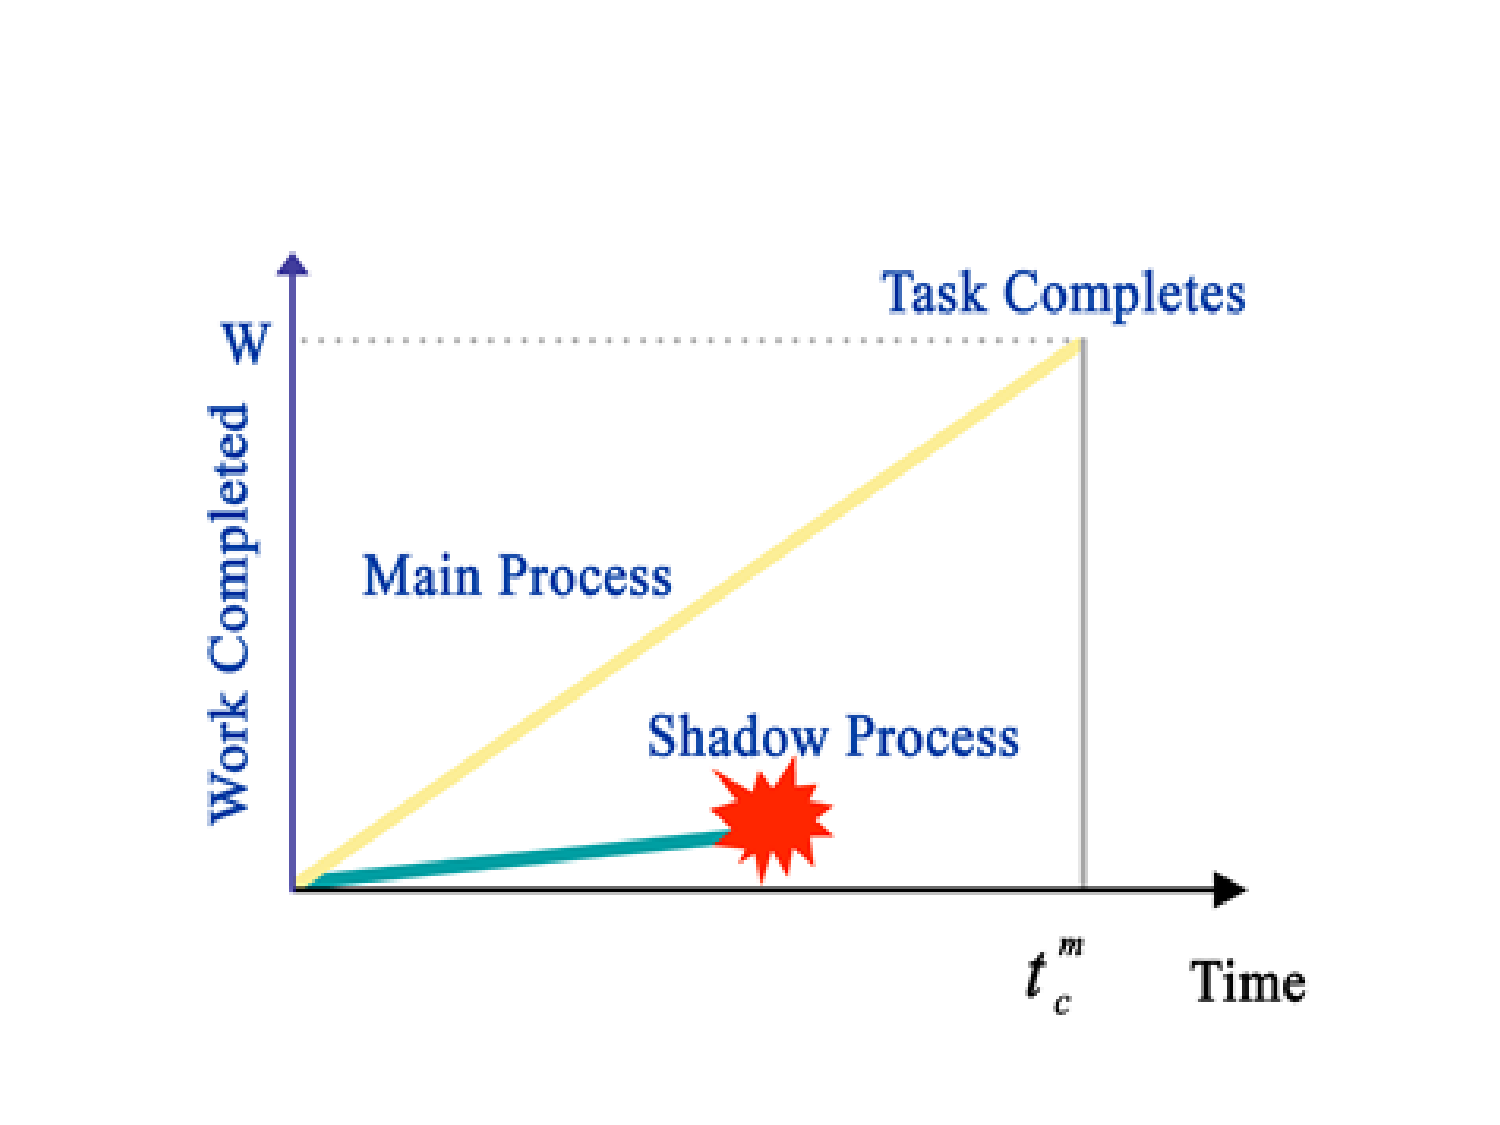
\includegraphics[width=0.28\textwidth]{figures/example3.pdf}
		}
		\subfigure[Main Process Failure]
		{
			\label{fig:sc_main_fail}
			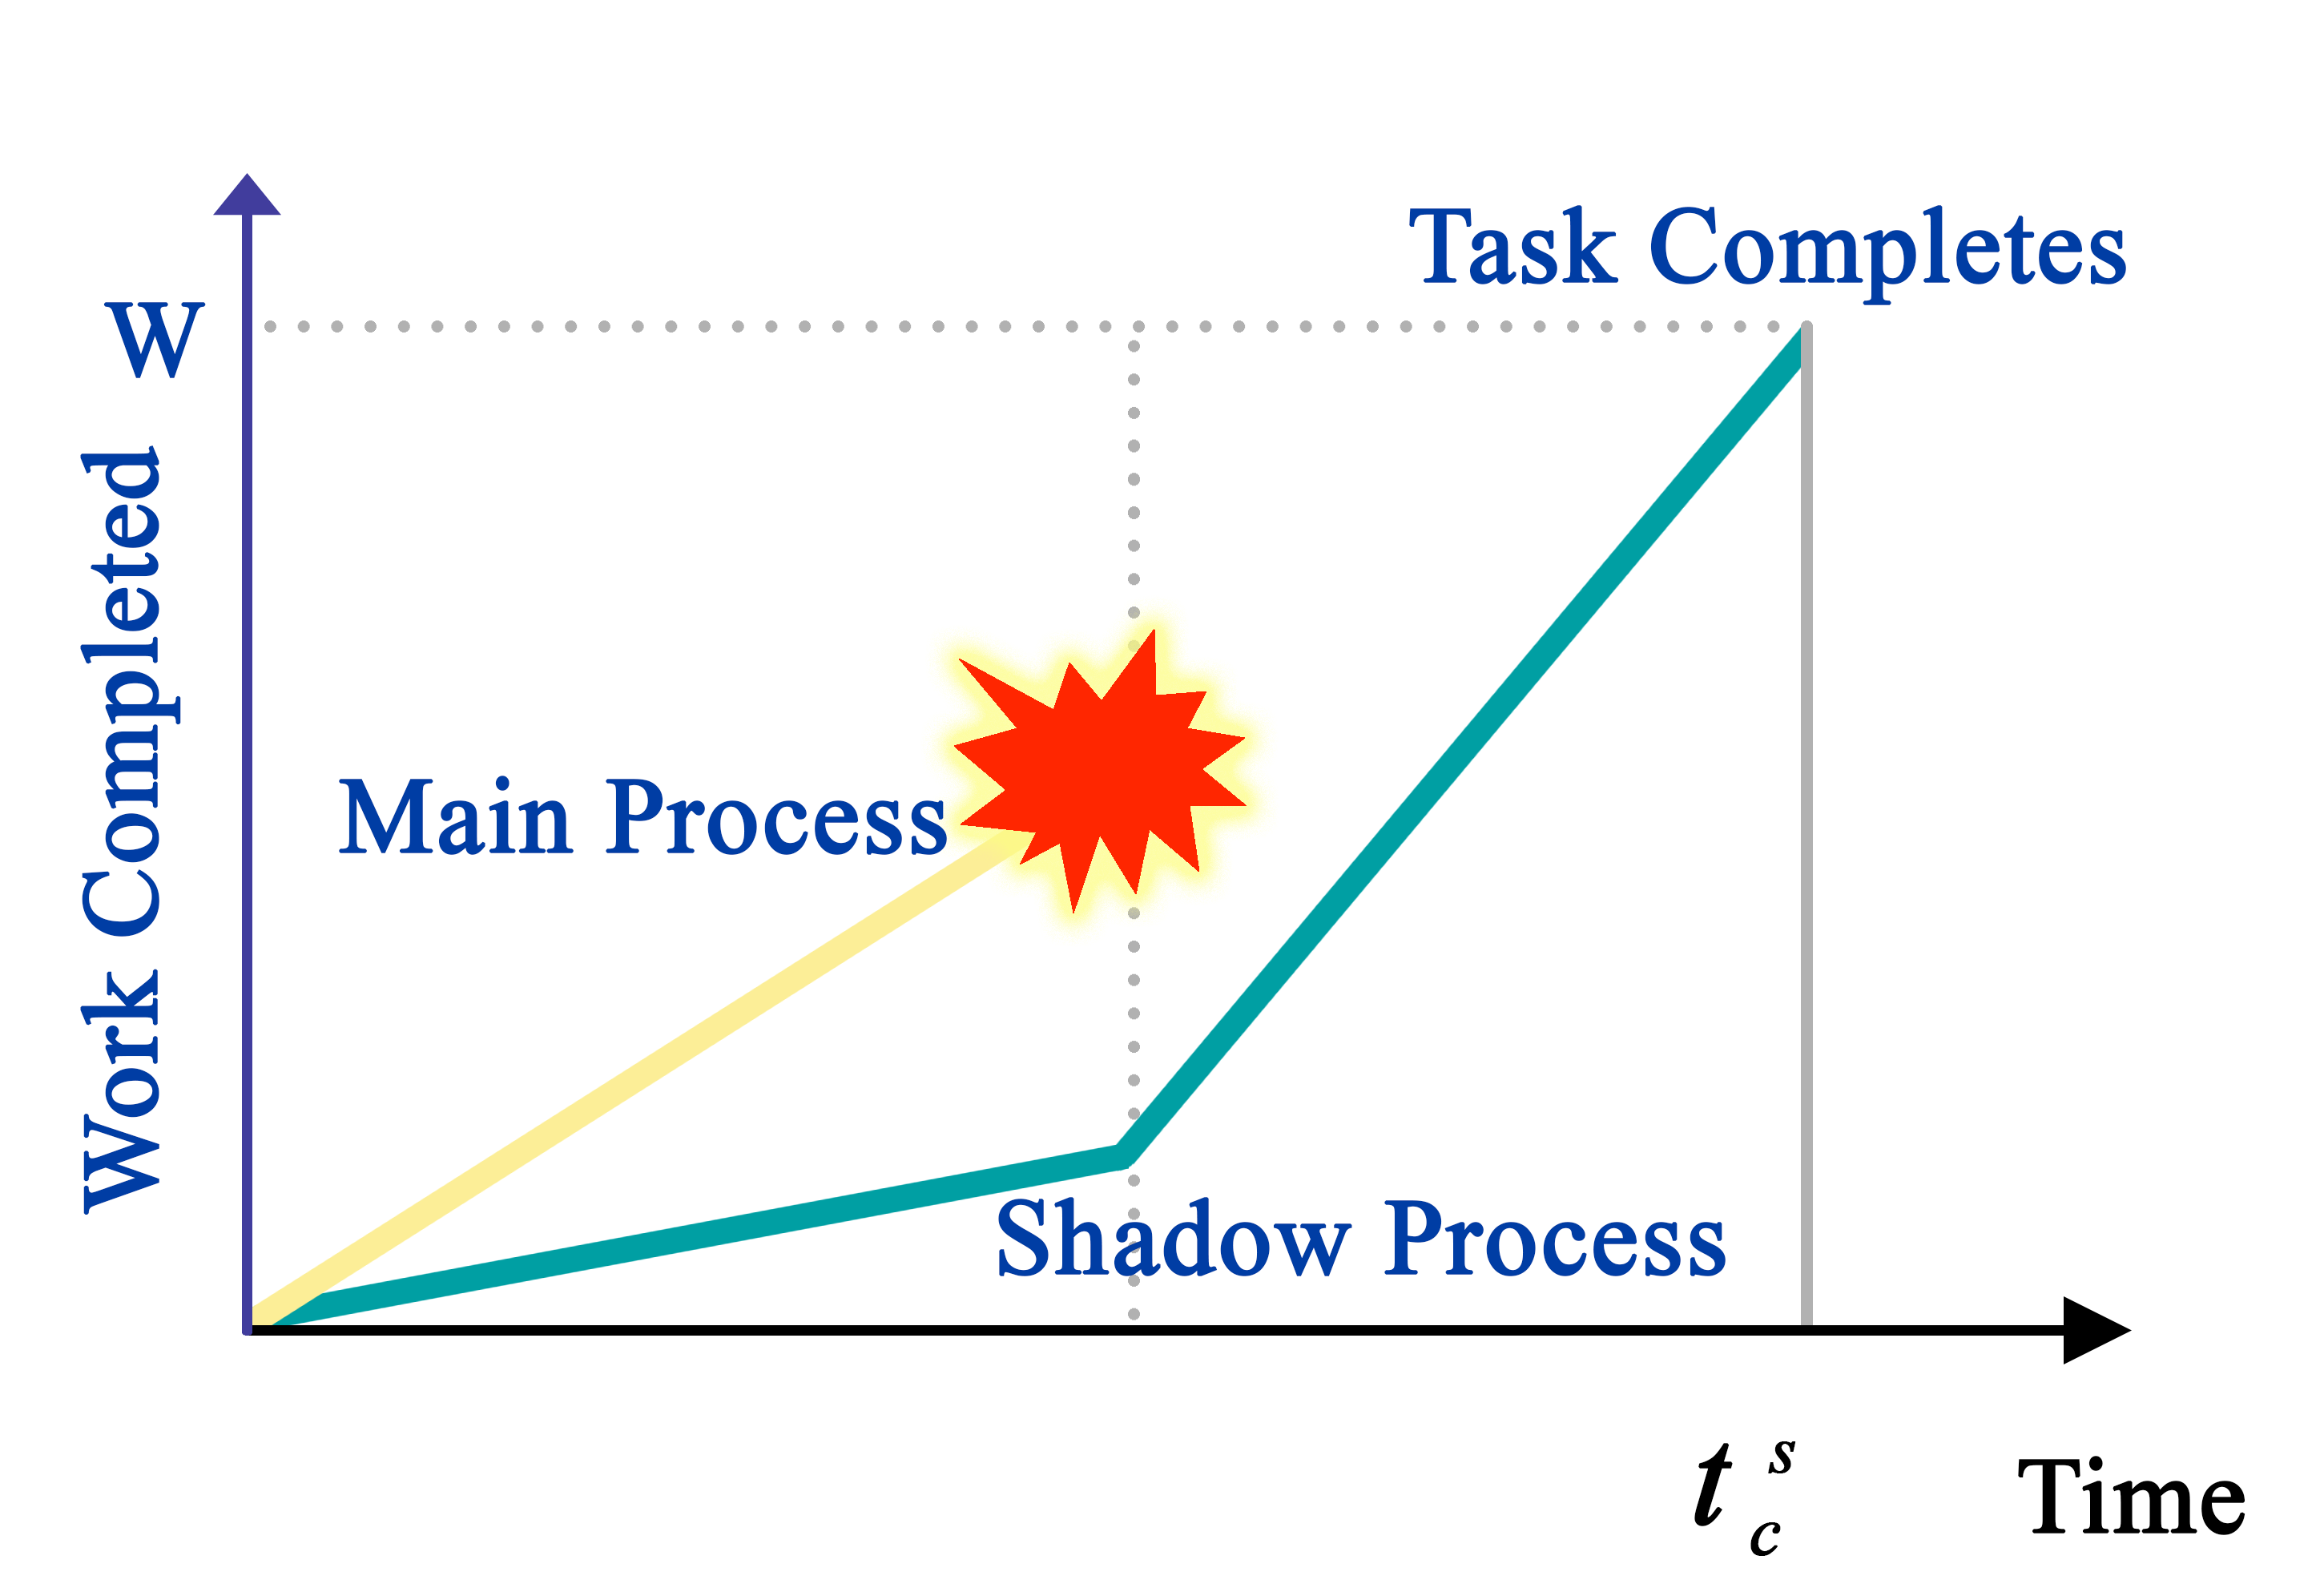
\includegraphics[width=0.32\textwidth]{figures/example2.png}
		}
	\end{center}
	\caption{Shadow Replication for a single task and single replica}
	\label{fig:sc_overview}
\end{figure}

Assuming a single process failure, Figure \ref{fig:sc_overview} illustrates the behavior of Shadow Replication with one shadow per task. 
%To illustrate the behavior of Shadow Replication, we limit the number of shadows to a single process and consider the scenarios depicted in Figure \ref{fig:sc_overview}, assuming a single process failure. 
If the main process does not fail, it will complete the task ahead of its shadow at $t_c^m$. At this time, we terminate the shadow immediately to save power. If the shadow fails before the main completes, the failure has no impact on the progress of the main. If the main fails, however, the shadow switches to a higher speed and completes the task at time $t_c^s$. 
%Figure \ref{fig:sc_no_fail} represents the case when neither the main nor the shadow fails. The main process, executing
%at a higher speed, completes the task at time $t_c^m$. At this time, the shadow process, progressing at a lower speed, stops execution immediately. Figure \ref{fig:sc_shadow_fail} represents the case when the shadow fails. This failure, however, has no impact on the progress of the main process, which still completes the task at $t_c^m$. Figure \ref{fig:sc_main_fail} depicts the case when the main process fails while the shadow is in progress. After detecting the failure of the main process, the shadow begins execution at a higher speed, completing the task at time $t_c^s$. 
Given that the failure rate of an individual node is much lower than
the aggregate system failure, it is very likely that the main process
will always complete its execution successfully, thereby achieving fault tolerance at a significantly reduced cost of energy consumed by the shadow. %saving a lot of energy for its associated shadow processes. 


A closer look at the model reveals that Shadow
Replication is a generalization of traditional fault tolerance
techniques, namely re-execution and process replication. If it allows for flexible completion time, 
Shadow Replication converges to re-execution as
the shadow remains idle during the execution of the main process and
only starts execution upon failure. If the target response time is
stringent, however, Shadow Replication converges to process replication,
as the shadow must execute simultaneously with the main at the same
speed. The flexibility of the Shadow Replication model provides the
basis for the design of a fault tolerance strategy that strikes a
balance between task completion time and energy saving. 

%Given that the probability of two individual nodes executing the same
%instances of a task fail at the same time is low, we will focus on the study of Shadow Replication model with a single shadow. It is clear, however, that the model can
%be extended to support multiple processes, as required by the
%application's fault-tolerance requirement. Furthermore, we adopt the
%fail-stop~ fault model, where a processor stops execution once a fault
%occurs and failure can be detected by other
%processes\cite{gartner_faults_1999,cristian_comm_1991}.

Based on DVFS, Mills studied the computational model in HPC systems and  
demonstrated that Shadow Replication can achieve resilience more efficiently than both checkpointing and process replication when power is limited~\cite{mills_2014_icnc,mills_2014_pdp,mills2014power}.
I am going to extend the work to achieve better flexibility, adaptivity, and scalability. 



